\section{Semi discrete Optimal Transport}

This tour treated the case when one of the measure was discrete while the other had a continuous density. The primal and the dual reads: 
\begin{align*}
    W_c(\alpha,\beta) &= \umin{\pi} \cb{
    \int_{\XY} c(x, y) \dd \pi(x,y) : \pi_1 = \alpha, \pi_2 = \beta
    } \\
    W_c(\alpha, \beta &= \umax{f, g} \cb{
    \int_\XX f(x) \dd \alpha (x) + \int_\YY g(y) \dd \beta (y) : f(x) + g(y) \leq c(x,y)
    }
\end{align*}

If $\alpha \sum_i a_i \delta_{x_i}$ and we replace $g$ by its $c$ transform, we obtain the following problem which is much more tractable:

\begin{equation}
\label{score_lagrangien}
    W_c(\alpha, \beta = \umax{f} \cb{
    \sum_i f(x_i) a_i + \int_\YY f^c(y) \dd \beta (y)
    }
\end{equation}

The $c$-transform of the discrete measure is a piece-wise smooth function on the \textbf{Laguerre} cells, defined by:

\begin{equation}
    L_i(f) \eqdef \cb{y \; | \; \forall j, c(x_i,y) - f_i \leq c(x_j,y) - f_j }
\end{equation}

Differentating the score defined in (\ref{score_lagrangien}), we obtain: 

\begin{equation}
    \partial_i E = a_i + \int_{L_i} f^c(y) \dd \beta(y)
\end{equation}

\subsection{Idea}

I lacked inspiration for this one, and got my idea from the news\footnote{\href{https://www.lemonde.fr/afrique/article/2019/12/09/madagascar-organise-une-concertation-nationale-sur-les-iles-eparses_6022235_3212.html}{Le Monde, \textit{Madagascar organise une concertation nationale sur les îles Eparses}}}. Madagascar is indeed claiming the ownership of the Scattered Island over France, which are a key strategic point, granting a large area of exclusive economic zone. I am not siding with any, but I was wondering how would look an \textbf{optimal assignment of sea resources} in that case. Indeed, we might want that all sides have equal access to the resources available; taking into consideration the distance between the land and the sea amounts to solving a transport problem. 

I did not spent too much time on this problem: it is directly an application of the notebook and does not explore mathematical ideas. Thus, the presented results could be easily optimized in various ways. 

\subsection{Data}

The \texttt{oceansdb} offers a database of the \textbf{tomography} of the oceans. We use a snapshot of the zone of interest, shown fig. \ref{fig:initial_map}. The discrete measure $\alpha$ represents points affiliated to the country in place. For big land part, I used multiple points; this could be improved by changing the distance between a point and the land. The continuous measure is simply the tomography of the ocean, ie. the ocean's depth. Indeed, we can model the \textbf{level of resources} with the \textbf{ocean's depth}. 

On a first try, I used:
\begin{equation}
\label{eq:depth}
    \beta (y) = \mathrm{depth}\, (y)
\end{equation}
ie. the deeper the ocean, the more resources there are. On a second try, I used a Gaussian kernel centered on -1000m, to give less importance to parts which are too deep or too shallow. It seems that around 1000m under the level of water, one can start finding rare metals and still be able to exploit them\footnote{Again, this is just an example and does not reflect my views or motivations!} \footnote{\href{https://www.nationalgeographic.com/environment/habitats/ocean/}{National Geographics: the Ocean}}. 

\begin{equation}
\label{eq:gaussian_depth}
    \beta (y) = \exp\p{-\frac{\mathrm{depth}\,(y) - \mu}{2 \sigma^2}}
\end{equation}

\begin{figure}[h]
    \centering
    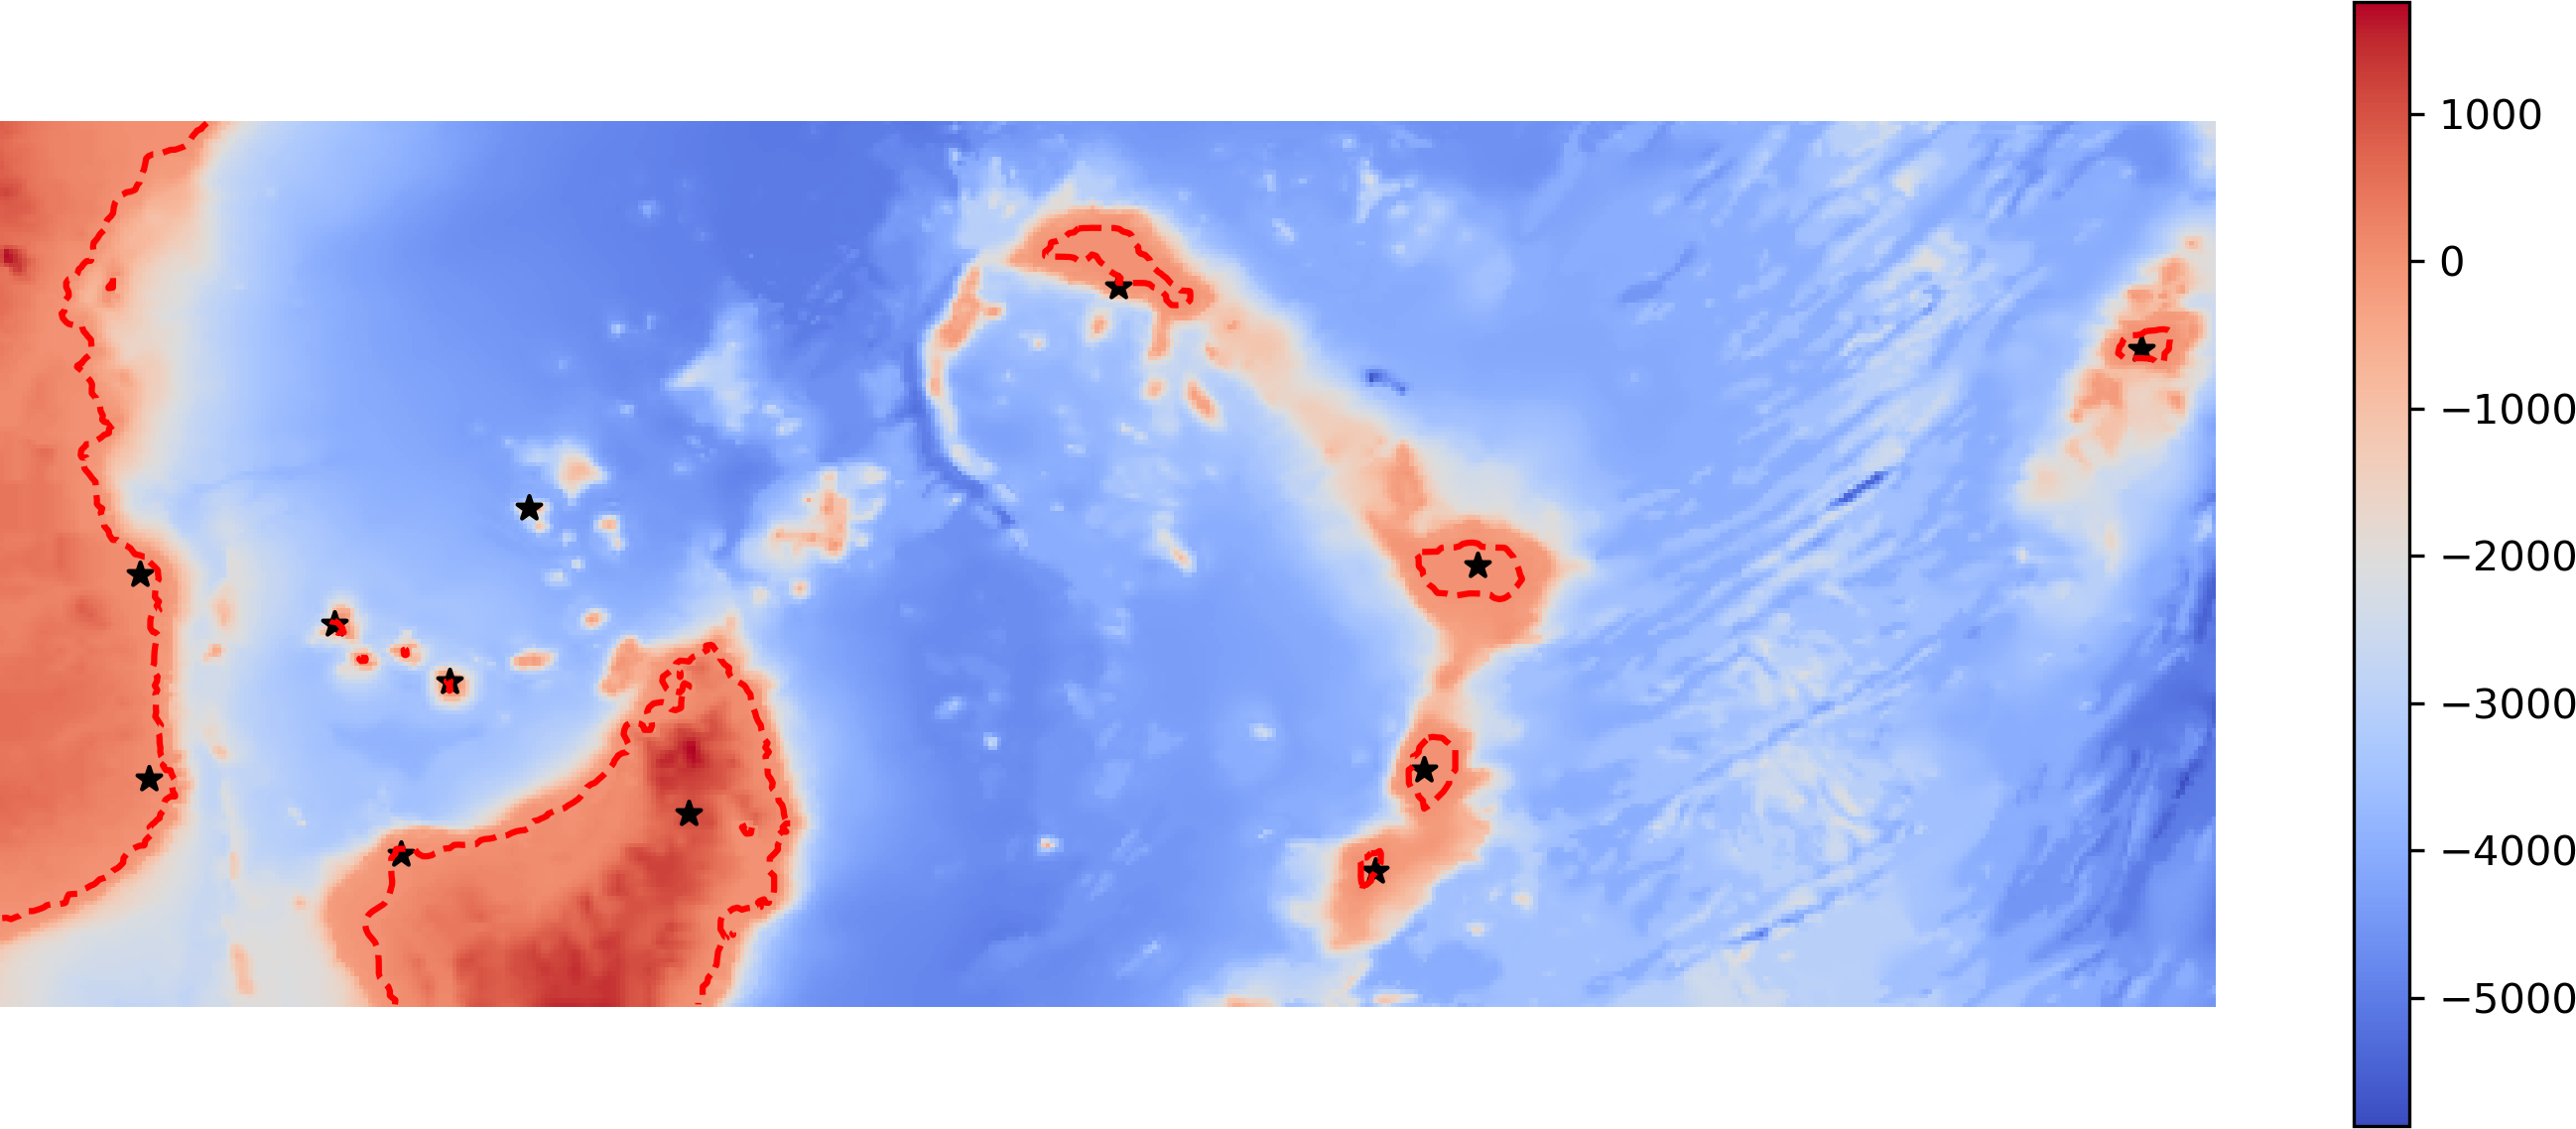
\includegraphics[width=.7\textwidth]{samples/3/starting_image.png}
    \caption{The area we are interested in, between latitude (-2, 19), and longitude (38, 73). On the west, the Mozambique. On the center, Madagascar. On the right, Seychelles and an island belonging to the UK. The Scattered Island are a few miles north of Madagascar. The support of the discrete measure are the 10 points scattered across the picture. The continuous measure (ie the ocean's tomography) is sampled on a fine grid of size (500, 300).}
    \label{fig:initial_map}
\end{figure}

\subsection{Gradient ascent}

The optimization problem (\ref{score_lagrangien}) can be solved by gradient ascent. Here, the number of variable is low so I did not notice any improvement in running a stochastic gradient ascent instead. The evolution of the Laguerre maps are shown fig. \ref{fig:evolution_laguerre_maps} and the dual value are fig. \ref{fig:evolution_lagrange_dual}.

\begin{figure}[p]
    \centering
    \begin{subfigure}[t]{.48\textwidth}
        \centering
        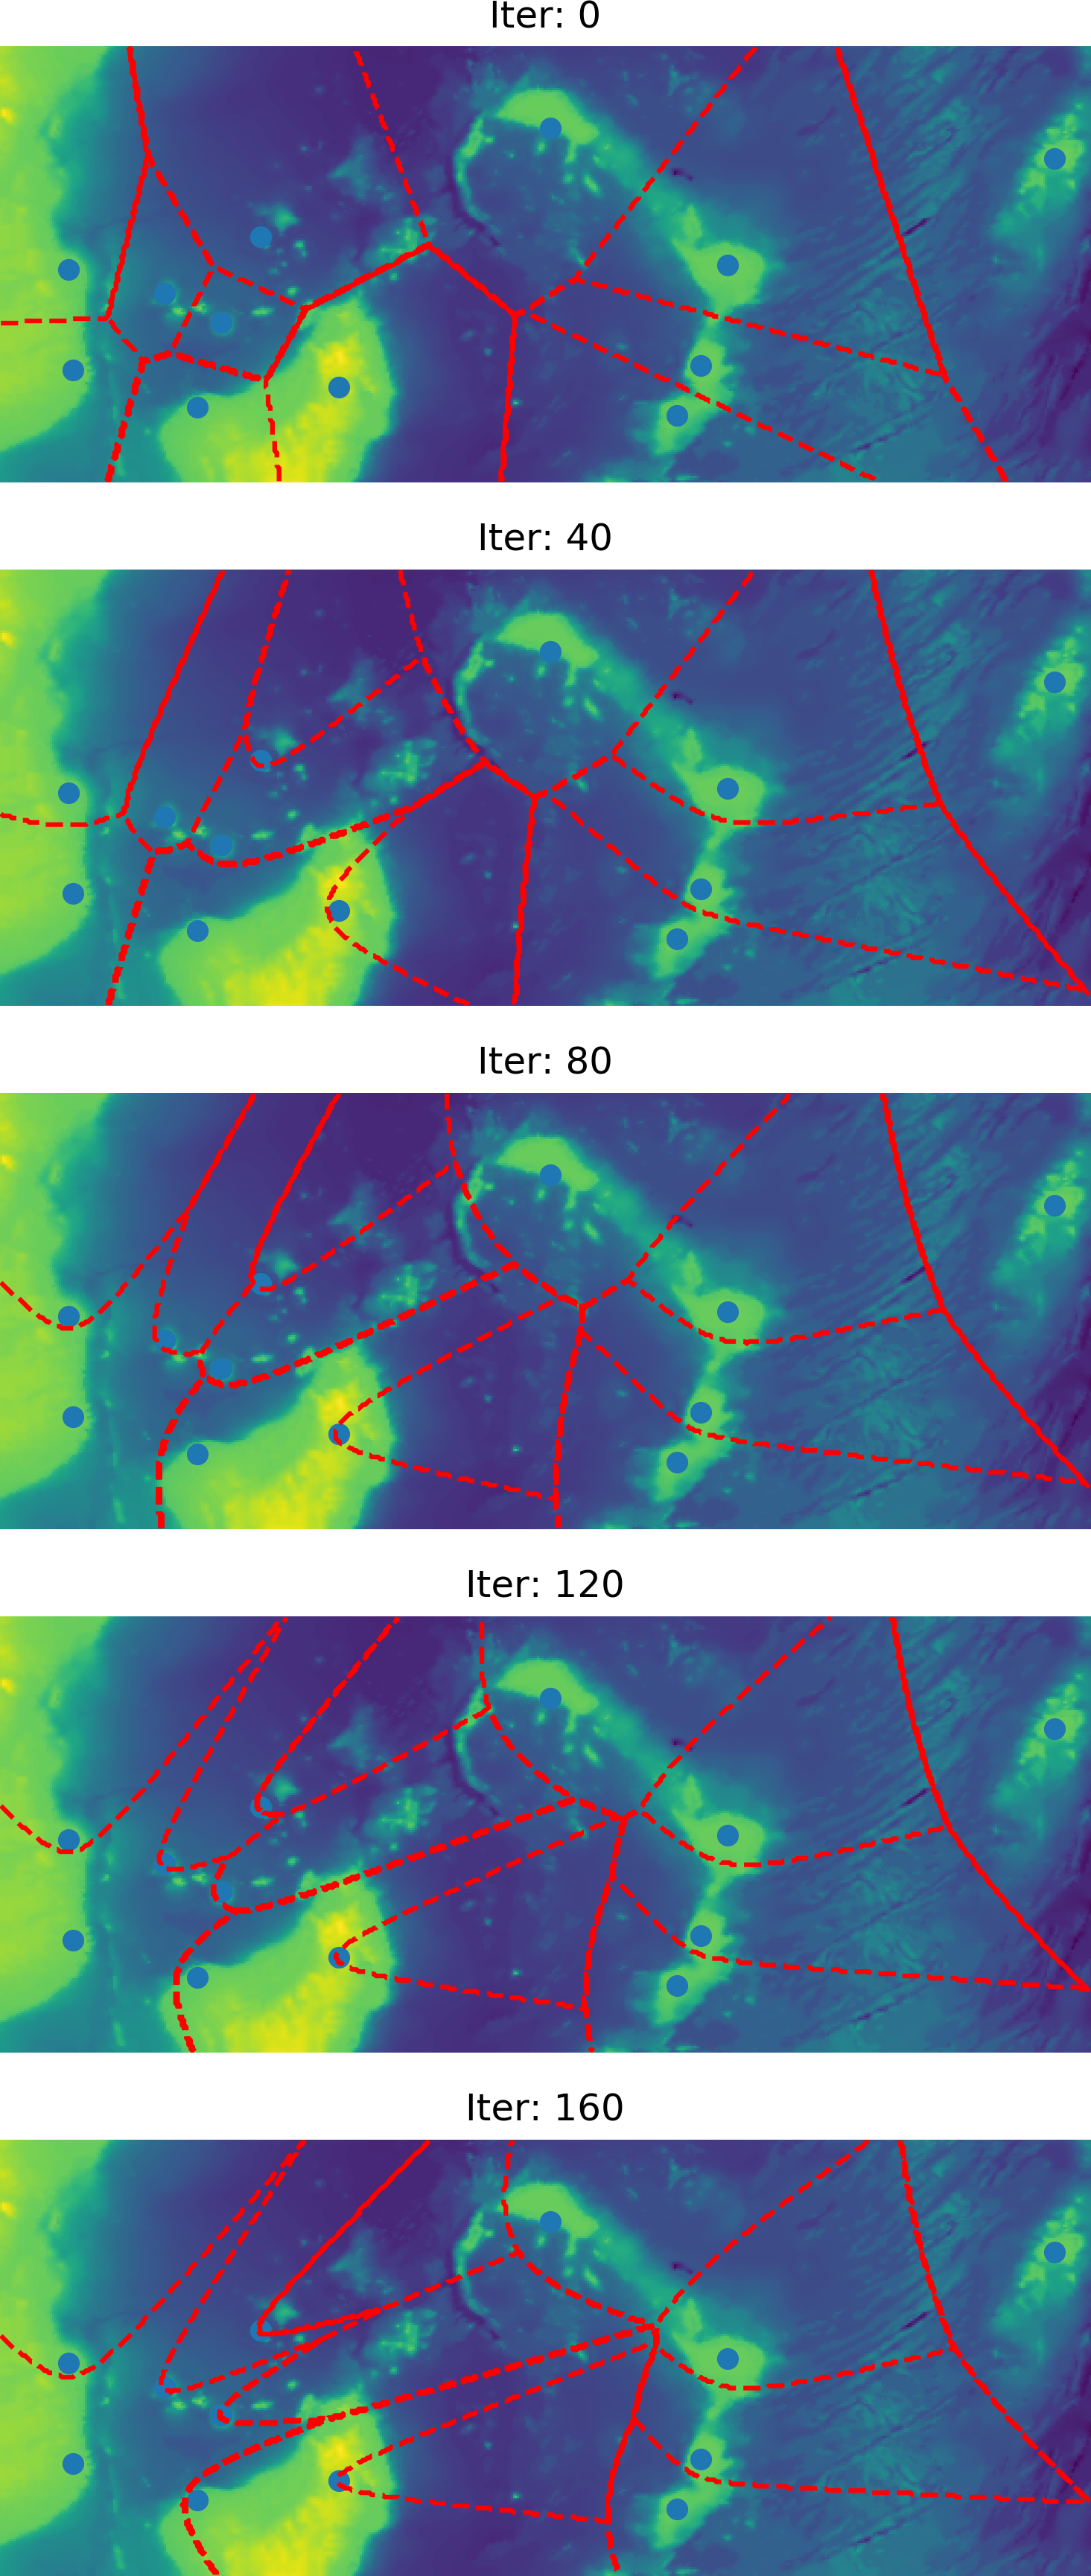
\includegraphics[width=\textwidth]{samples/3/repartition_evolution_true.png}
        \caption{With depth as the measure $\beta$ (eq. \ref{eq:depth}).}
    \end{subfigure}
    \hfill
    \begin{subfigure}[t]{.48\textwidth}
        \centering
        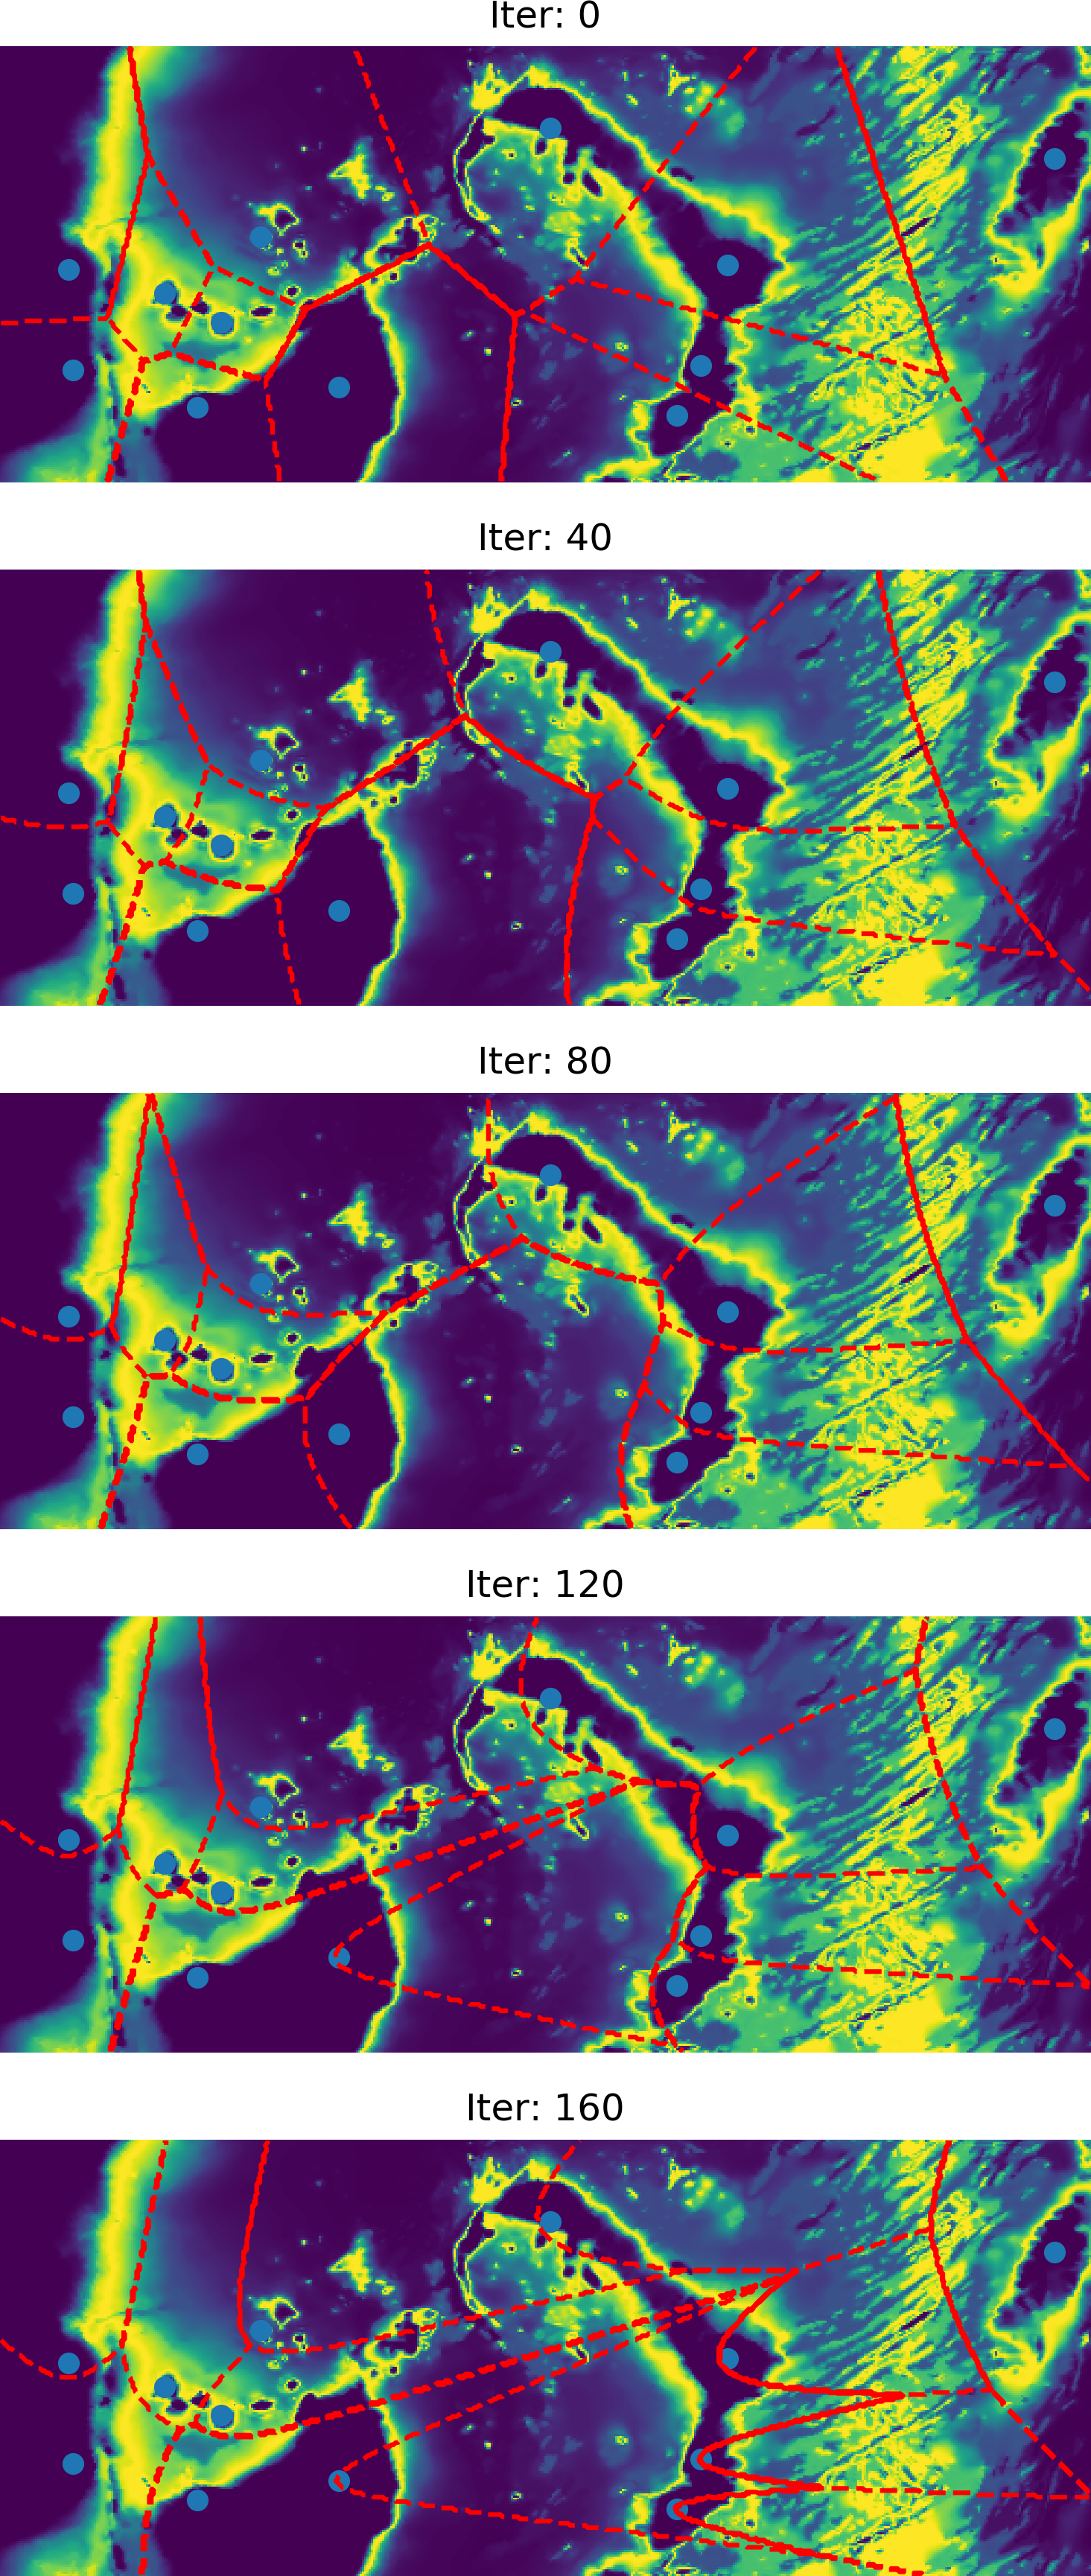
\includegraphics[width=\textwidth]{samples/3/repartition_evolution_gaussian.png}
        \caption{With a Gaussian kernel on depth as the measure $\beta$ (eq. \ref{eq:gaussian_depth}).}
    \end{subfigure}
    \caption{Evolution of the Laguerre maps during the gradient ascent, with two different measure for $\beta$.}
    \label{fig:evolution_laguerre_maps}
\end{figure}

\begin{figure}[p]
    \centering
    \begin{subfigure}[c]{.4\textwidth}
        \centering
        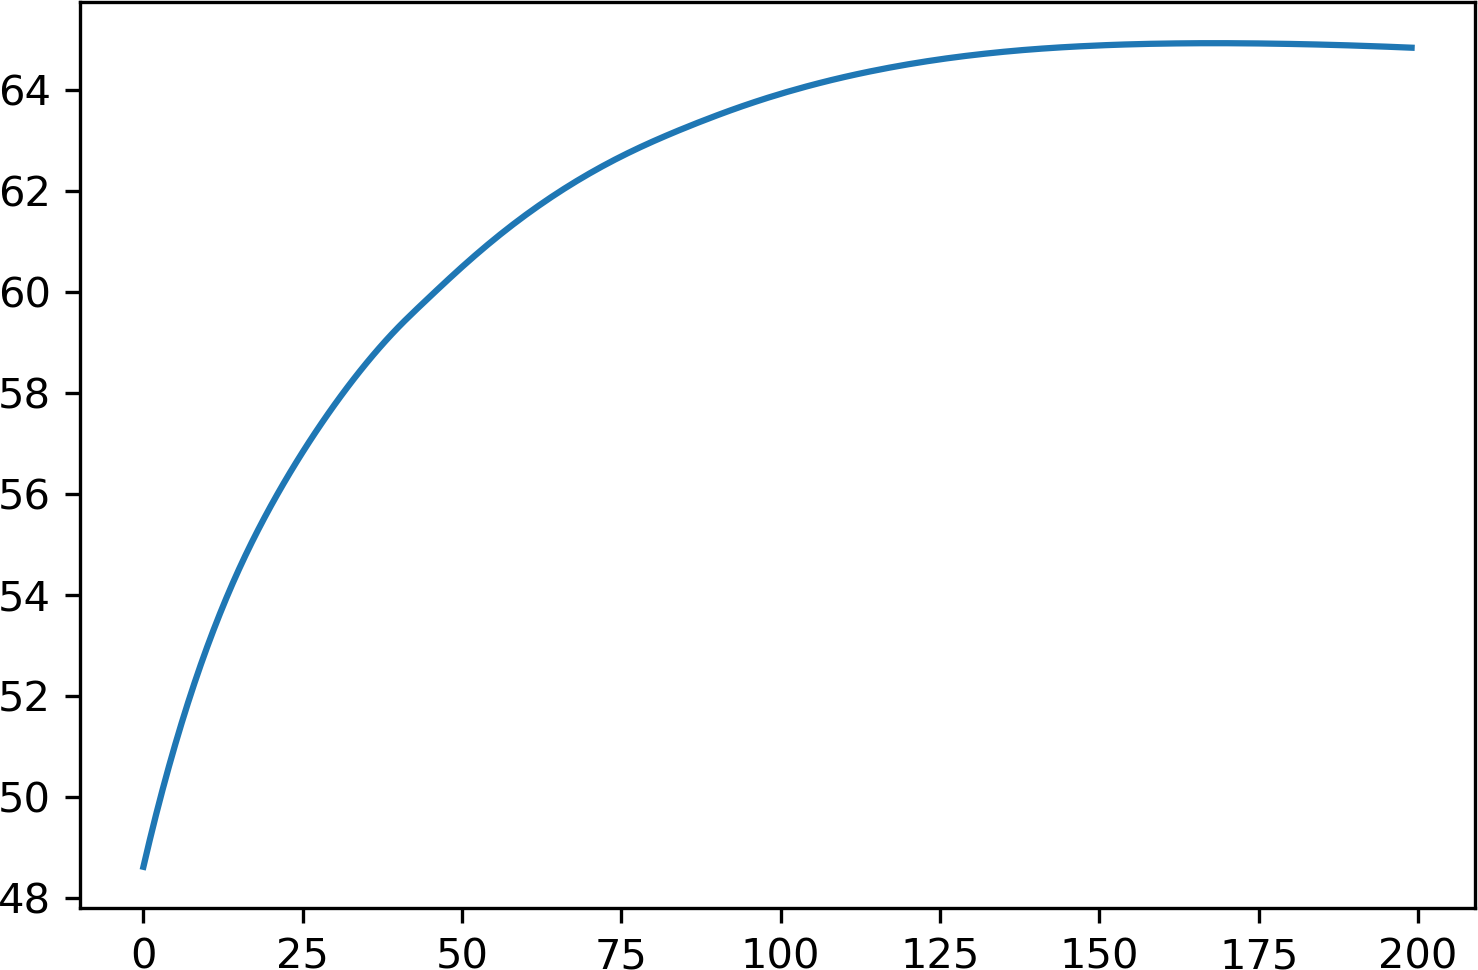
\includegraphics[width=\textwidth]{samples/3/evolution_of_dual_value_TRUE.png}
        \caption{With depth as the measure $\beta$ (eq. \ref{eq:depth}).}
    \end{subfigure}
    \hfill
    \begin{subfigure}[c]{.4\textwidth}
        \centering
        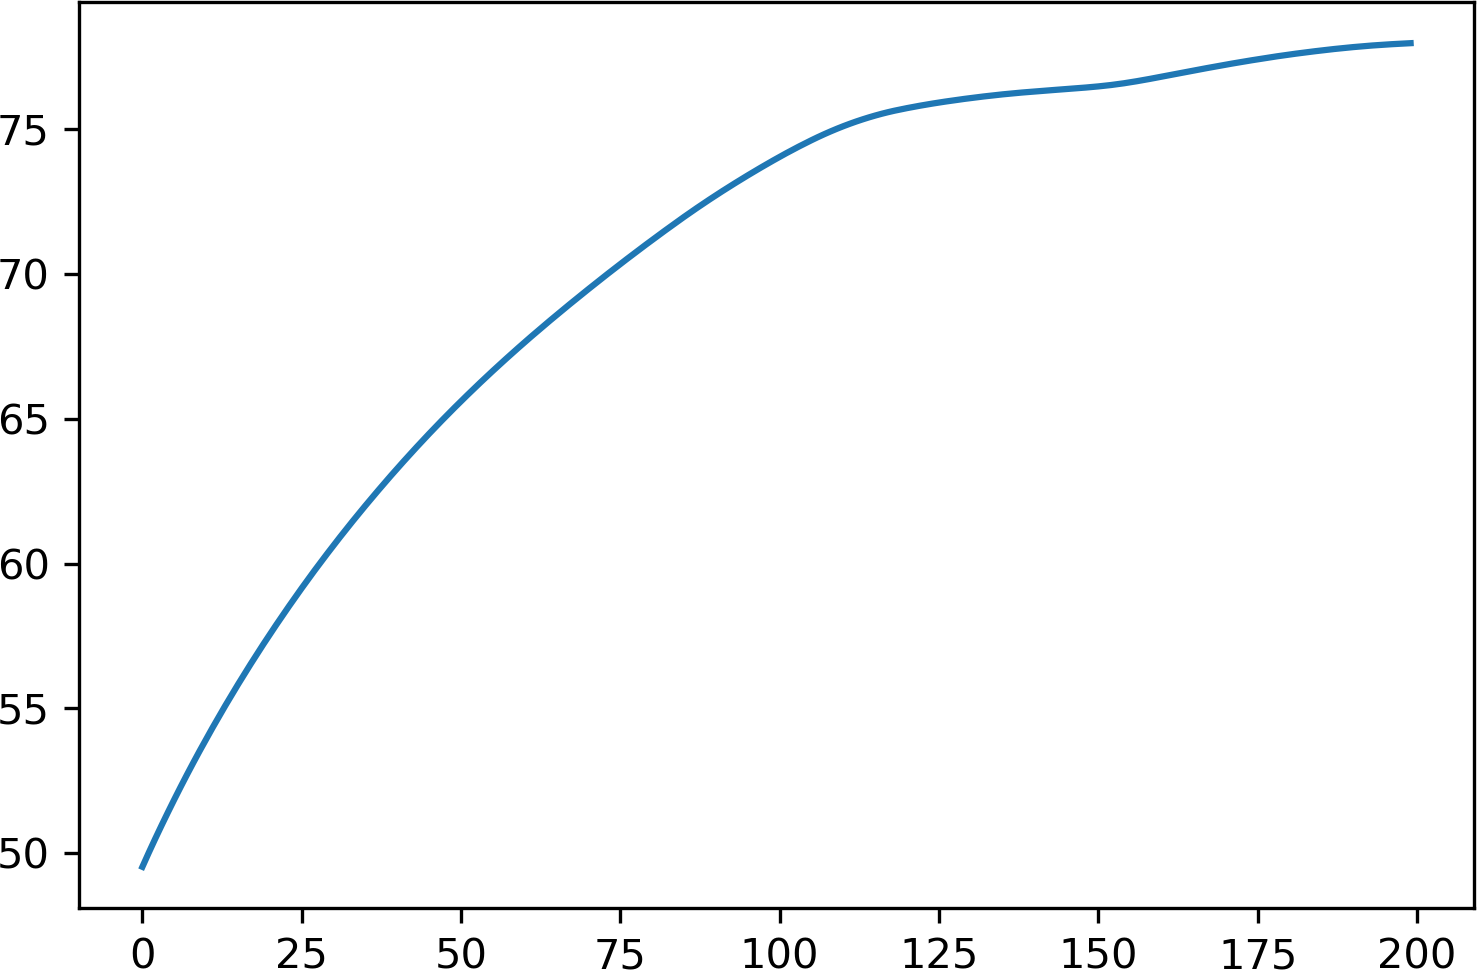
\includegraphics[width=\textwidth]{samples/3/evolution_of_dual_value_gaussian.png}
        \caption{With a Gaussian kernel on depth as the measure $\beta$ (eq. \ref{eq:gaussian_depth}).}
    \end{subfigure}
    \caption{Evolution of the dual value during the gradient ascent, with two different measure for $\beta$.}
    \label{fig:evolution_lagrange_dual}
\end{figure}

\subsection{Results}

Finally, the results are shown fig. \ref{fig:part3_final_results}. Of course, they are terrible. But I find it still satisfying to know that each of these color players have an equal access to the ocean's resources. If we had taken a better distance, e.g. one which would compute the smallest distance to a point on the land, we would not have the Madagascar Island cut this way.

\begin{figure}[h]
    \centering
    \begin{subfigure}[c]{.9\textwidth}
        \centering
        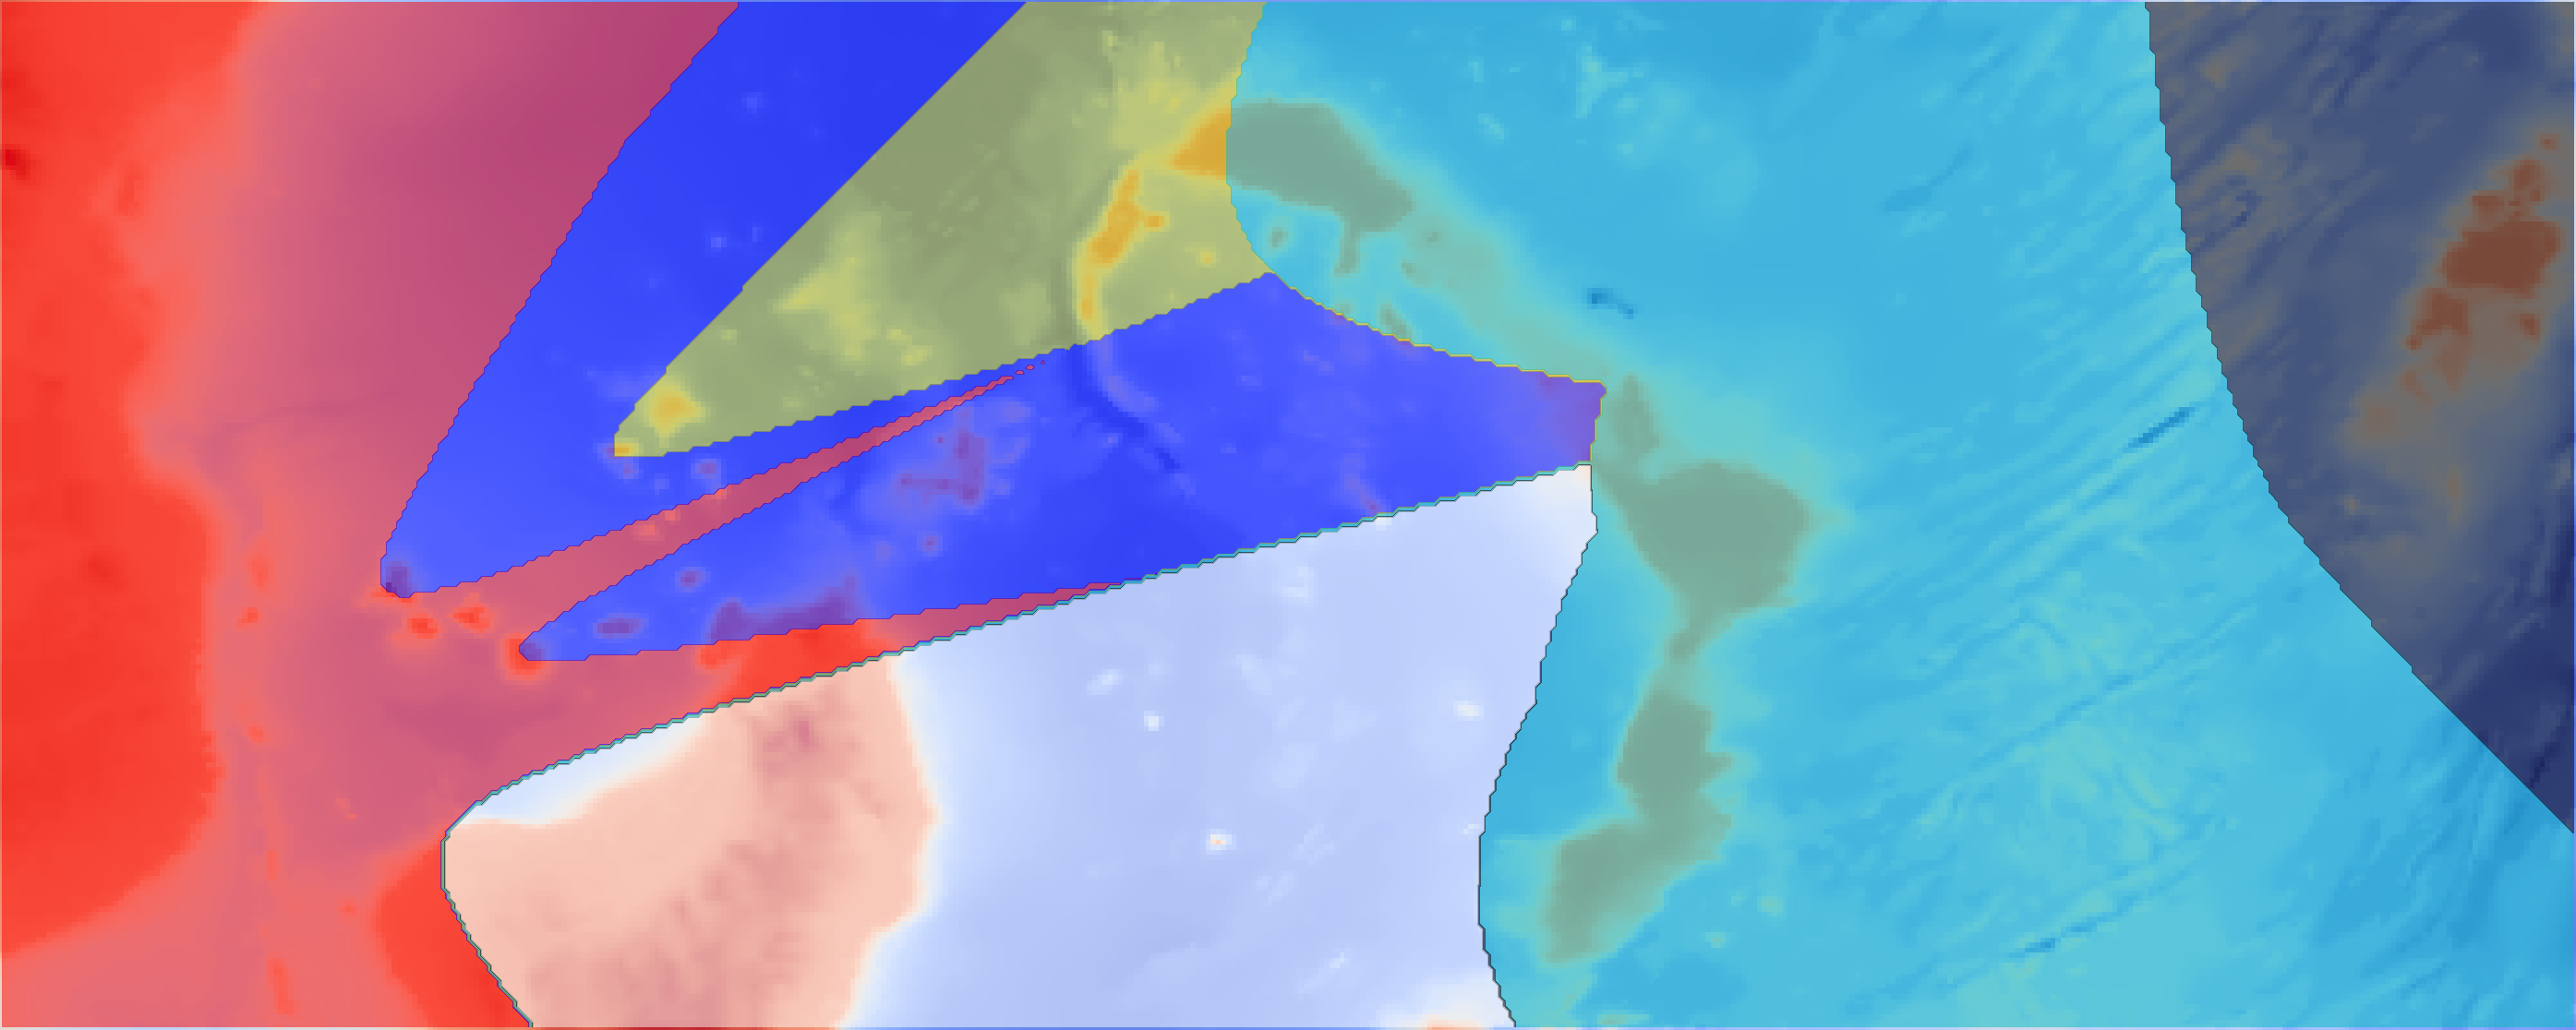
\includegraphics[width=\textwidth]{samples/3/final_map_true.png}
        \caption{With depth as the measure $\beta$ (eq. \ref{eq:depth}).}
    \end{subfigure}
    
    \begin{subfigure}[c]{.9\textwidth}
        \centering
        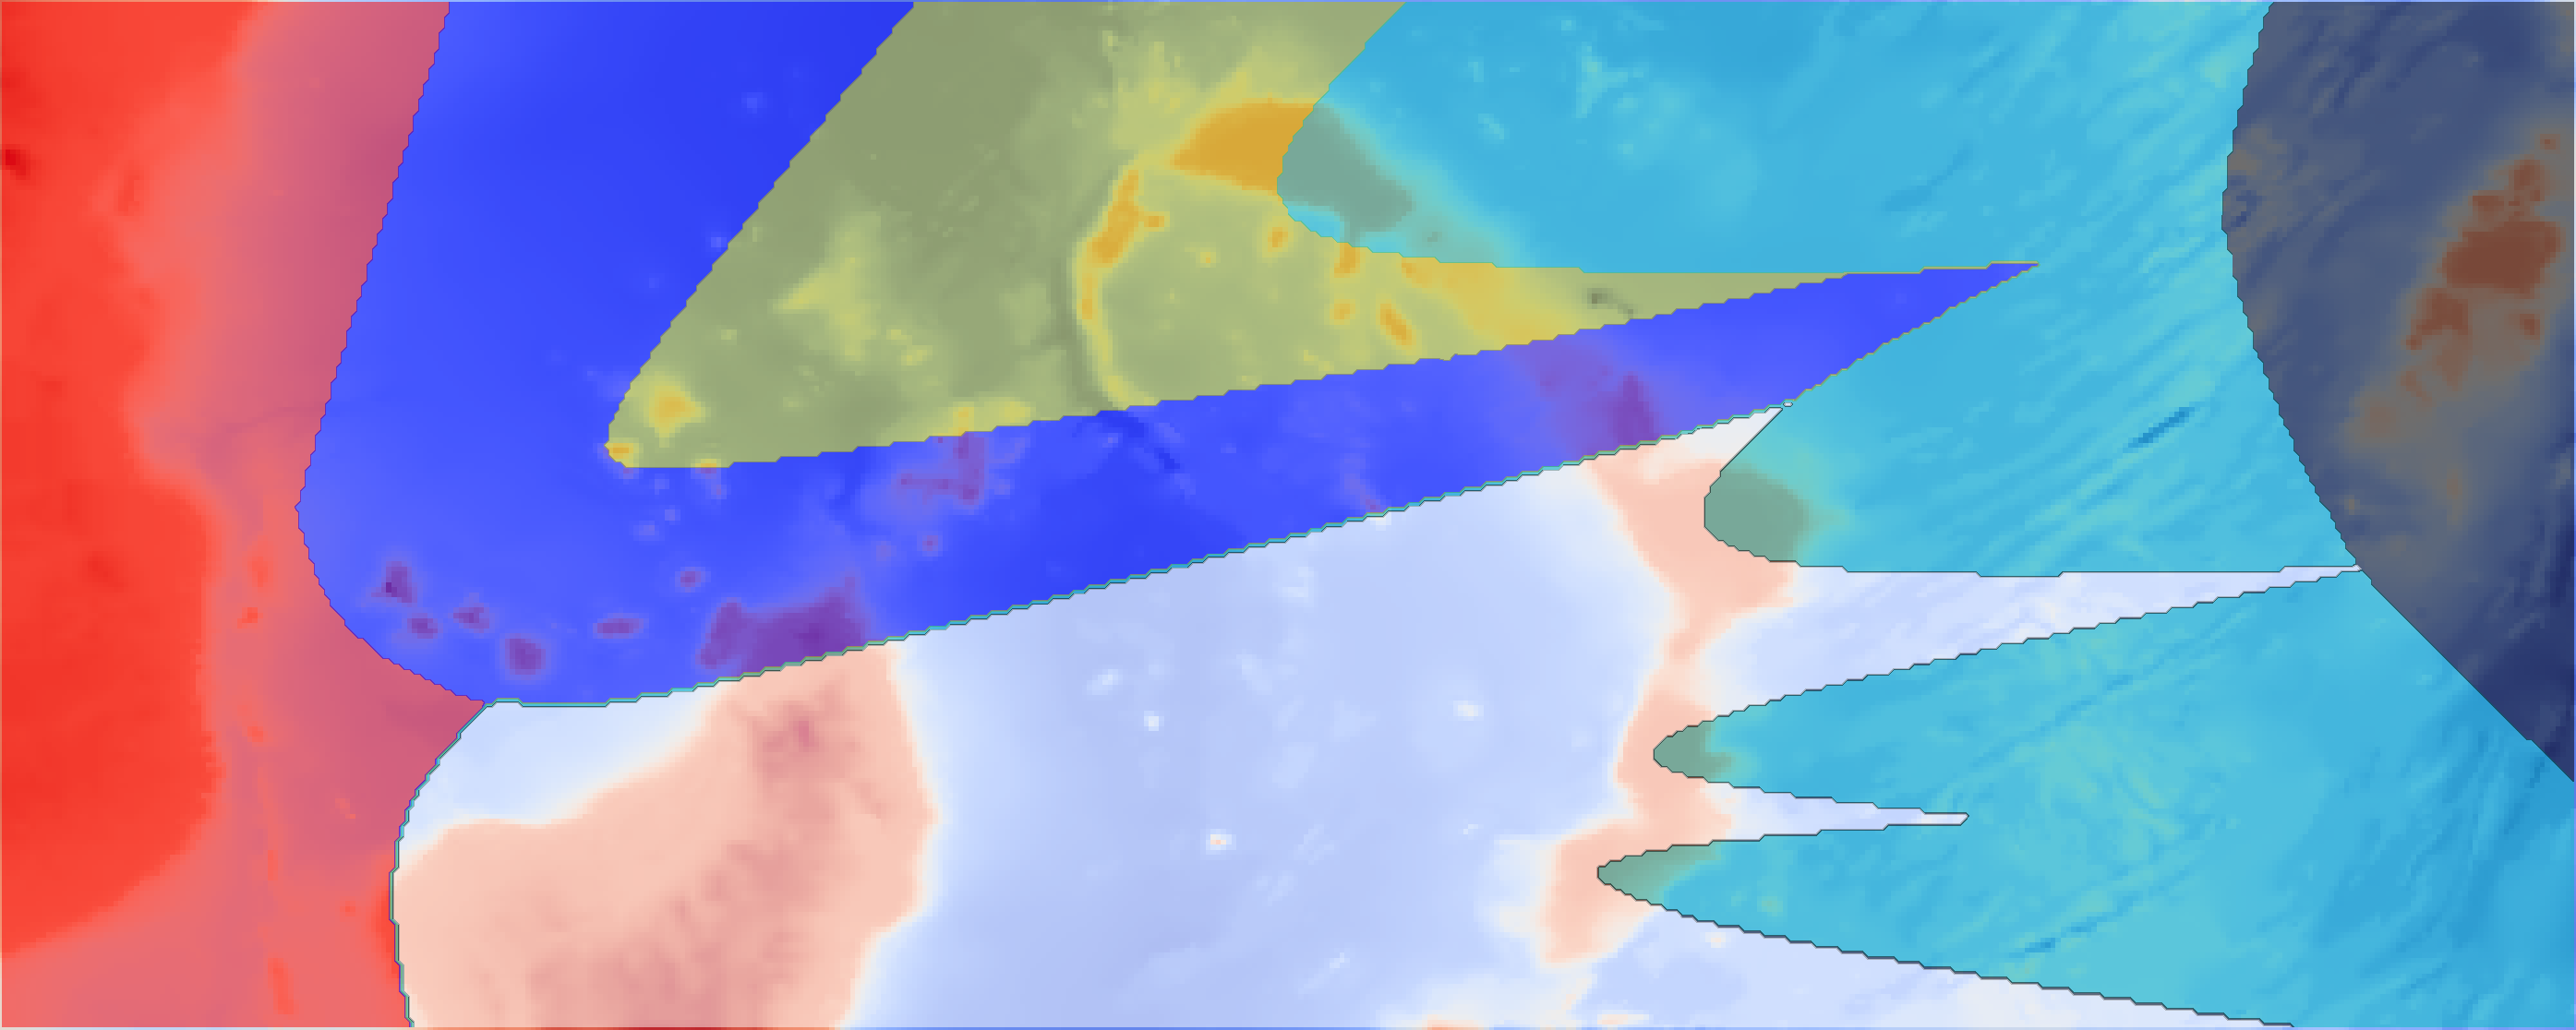
\includegraphics[width=\textwidth]{samples/3/final_map_gaussian.png}
        \caption{With a Gaussian kernel on depth as the measure $\beta$ (eq. \ref{eq:gaussian_depth}).}
    \end{subfigure}
    \caption{Final coupling found by dual ascent, for two different kind of distribution $\beta$.}
    \label{fig:part3_final_results}
\end{figure}

